% answers.tex —— 1985 年·广东卷·文史类 · 参考答案与详细解析片段
% 由 tools/generate_projects.py 依来源总账自 1985/1985_数学真题_广东文史类_试题.md + 1985/1985_数学真题_广东文史类_解析正文.md + 1985/1985_数学真题_广东文史类_答案要点.md 生成，勿手改（改源 MD 后重跑）


\begin{gktip}
本文给出独立推导；题面疑字见题面 U 标记。原书解答中的漏字、评分冲突与推理错误不作为证明依据。
\end{gktip}

\begin{answer}
\gksolhead{1}{卷一填空 1}

\textbf{题目}：

$log_3 5\cdot\log_5 9$ 的值等于＿＿。

\Needspace{4\baselineskip}
\textbf{解析}

由对数换底公式，$\log_3 5\cdot\log_5 9=\log_3 9$。

\gkanswer{答案：$2$}

\end{answer}
\begin{answer}
\gksolhead{2}{卷一填空 2}

\textbf{题目}：

设数列 ${a_n}$ 的首项 $a_1=8$，且 $a_n=2a_{n-1}\ (n=2,3,\ldots)$，则 $a_4$ 的数值是＿＿。

\Needspace{4\baselineskip}
\textbf{解析}

递推三次可得 $a_4=2^3a_1$。

\gkanswer{答案：$64$}

\end{answer}
\begin{answer}
\gksolhead{3}{卷一填空 3}

\textbf{题目}：

复数 $\sqrt3-i$ 的三角形式是＿＿。

\Needspace{4\baselineskip}
\textbf{解析}

复数模长为 $\sqrt{3+1}=2$，主辐角可取 $11\pi/6$。复数三角形式的正弦项必须带虚数单位 $i$。

\gkanswer{答案：$2\bigl(\cos\frac{11\pi}{6}+i\sin\frac{11\pi}{6}\bigr)$}

\end{answer}
\begin{answer}
\gksolhead{4}{卷一填空 4}

\textbf{题目}：

如果 $f(1/x)=x/(1-x^2)$，则 $f(x)=$＿＿。

\Needspace{4\baselineskip}
\textbf{解析}

令 $t=1/x$，原关系给出 $f(t)=(1/t)/(1-1/t^2)=t/(t^2-1)$。原条件中 $x\ne0,\pm1$，所以不能由此确定 $f(0)$。

\gkanswer{答案：$\dfrac{x}{x^2-1}$（题设仅确定 $x\ne0,\pm1$ 时的函数值）}

\end{answer}
\begin{answer}
\gksolhead{5}{卷一填空 5}

\textbf{题目}：

如果一个圆锥底面的半径增大到原来的 3 倍，但要保持它的体积不变，则其高必须缩小到原来的＿＿。

\Needspace{4\baselineskip}
\textbf{解析}

圆锥体积 $V=\pi r^2h/3$。半径乘 3 而体积不变，故高度乘 $1/9$。

\gkanswer{答案：$\dfrac19$}

\end{answer}
\begin{answer}
\gksolhead{6}{卷一填空 6}

\textbf{题目}：

$\cos(\pi/5)+\cos(2\pi/5)+\cos(3\pi/5)+\cos(4\pi/5)$ 的值等于＿＿。

\Needspace{4\baselineskip}
\textbf{解析}

利用 $\cos(\pi-\theta)=-\cos\theta$，第一项与第四项相消，第二项与第三项相消。

\gkanswer{答案：$0$}

\end{answer}
\begin{answer}
\gksolhead{7}{卷一填空 7}

\textbf{题目}：

$\displaystyle\lim_{n\to\infty}\frac{1+4+7+\cdots +(3n-2)}{n(n+1)}$ 的值等于＿＿。

\Needspace{4\baselineskip}
\textbf{解析}

等差数列求和得 $1+4+\cdots +(3n-2)=n(3n-1)/2$。代入原式后，极限为 $\lim_{n\to\infty}(3n-1)/(2n+2)$。

\gkanswer{答案：$\dfrac32$}

\end{answer}
\begin{answer}
\gksolhead{8}{卷一填空 8}

\textbf{题目}：

在一个长方体中，和其中一条确定的棱相垂直的棱的总数是＿＿条。

\Needspace{4\baselineskip}
\textbf{解析}

长方体的棱按方向分为三组，每组 4 条。与指定棱同方向的 4 条不垂直，其余两组共 8 条；若把“垂直”严格限定为相交，计数口径需另行确认（U08）。

\gkanswer{答案：$8$（按棱的垂直方向计数；若“垂直”限于相交则为 4，见 U08）}

\end{answer}
\begin{answer}
\gksolhead{9}{卷一填空 9}

\textbf{题目}：

双曲线 $x^2/3-y^2=1$ 的两条渐近线所夹的锐角的大小是＿＿弧度。

\Needspace{4\baselineskip}
\textbf{解析}

渐近线为 $y=\pm x/\sqrt3$，分别与正 $x$ 轴成 $\pm\pi/6$，两线的锐夹角是 $\pi/3$。

\gkanswer{答案：$\dfrac\pi3$ 弧度}

\end{answer}
\begin{answer}
\gksolhead{10}{卷一填空 10}

\textbf{题目}：

函数 $y=\sin^2(2x)$ 的最小正周期是＿＿。

\Needspace{4\baselineskip}
\textbf{解析}

$\sin^2(2x)=[1-\cos(4x)]/2$。余弦项的周期为 $2\pi/4$，且系数非零，故这也是原函数的最小正周期。

\gkanswer{答案：$\dfrac\pi2$}

\end{answer}
\begin{answer}
\gksolheadwithlabel{11}{1}{卷一选择 1}

\textbf{题目}：

函数 $y=2^{-x}$ 的图象的大致形状是：A 递增指数曲线，过 $(0,1)$；B 第一象限递减曲线，图注 $(1,1)$；C 递减曲线，图注 $(1,0)$，穿过横轴；D 递增对数形曲线，过 $(1,0)$；E 递减指数曲线，过 $(0,1)$。
\nopagebreak[4]
\begin{center}% 1985 广东文史类卷一二（1）：五幅指数/对数函数候选图；仅示意曲线形状。
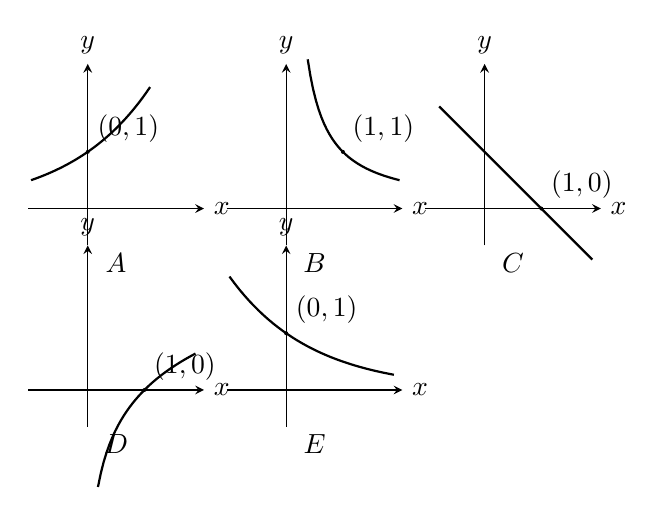
\begin{tikzpicture}[scale=0.72,>=stealth]
  \foreach \x/\y/\label in {0/0/A,3.5/0/B,7/0/C,0/-3.2/D,3.5/-3.2/E} {
    \begin{scope}[shift={(\x,\y)}]
      \draw[->] (-1.05,0)--(2.05,0) node[right] {$x$};
      \draw[->] (0,-0.65)--(0,2.55) node[above] {$y$};
      \node[below] at (0.5,-0.62) {$\label$};
    \end{scope}
  }
  % A：递增指数曲线，过 (0,1)
  \begin{scope}
    \draw[thick,domain=-1:1.1,samples=35] plot (\x,{2^\x});
    \fill (0,1) circle (1pt) node[above right] {$(0,1)$};
  \end{scope}
  % B：仅第一象限递减，标点 (1,1)
  \begin{scope}[shift={(3.5,0)}]
    \draw[thick,domain=0.38:2,samples=35] plot (\x,{1/\x});
    \fill (1,1) circle (1pt) node[above right] {$(1,1)$};
  \end{scope}
  % C：递减并穿过 (1,0)
  \begin{scope}[shift={(7,0)}]
    \draw[thick,domain=-0.8:1.9,samples=35] plot (\x,{1-\x});
    \fill (1,0) circle (1pt) node[above right] {$(1,0)$};
  \end{scope}
  % D：递增对数形曲线，过 (1,0)
  \begin{scope}[shift={(0,-3.2)}]
    \draw[thick,domain=0.18:1.9,samples=35] plot (\x,{ln(\x)});
    \fill (1,0) circle (1pt) node[above right] {$(1,0)$};
  \end{scope}
  % E：递减指数曲线，过 (0,1)，向右趋近 x 轴
  \begin{scope}[shift={(3.5,-3.2)}]
    \draw[thick,domain=-1:1.9,samples=35] plot (\x,{2^(-\x)});
    \fill (0,1) circle (1pt) node[above right] {$(0,1)$};
  \end{scope}
\end{tikzpicture}
\end{center}
\nopagebreak[4]
\Needspace{4\baselineskip}
\textbf{解析}

指数函数 $2^{-x}$ 对所有实数为正、严格递减，且经过 $(0,1)$；当 $x$ 增大时趋近于 $x$ 轴但不与之相交。依这些特征辨认图形。

\gkanswer{答案：E}

\end{answer}
\begin{answer}
\gksolheadwithlabel{12}{2}{卷一选择 2}

\textbf{题目}：

函数 $y=\sqrt{\lg(1-x)}$ 的定义域是：A $(-\infty,+\infty)$；B $(-\infty,0]$；C $(-\infty,0)$；D $(-\infty,1]$；E $(-\infty,1)$。

\Needspace{4\baselineskip}
\textbf{解析}

平方根要求 $\lg(1-x)\ge0$，即 $1-x\ge1$；同时真数为正已包含在此条件中。

\gkanswer{答案：B}

\end{answer}
\begin{answer}
\gksolheadwithlabel{13}{3}{卷一选择 3}

\textbf{题目}：

以 $A(1,3)$、$B(-5,1)$ 为端点的线段的垂直平分线方程是：A $3x-y+8=0$；B $3x+y+8=0$；C $2x-y-6=0$；D $2x+y+2=0$；E $3x+y+4=0$。

\Needspace{4\baselineskip}
\textbf{解析}

中点为 $(-2,2)$，直线 $AB$ 的斜率为 $1/3$，故垂直平分线斜率为 $-3$。用点斜式列直线方程。

\gkanswer{答案：E}

\end{answer}
\begin{answer}
\gksolheadwithlabel{14}{4}{卷一选择 4}

\textbf{题目}：

下列不等式中，成立的是：A $\sin(3\pi/8)<\sin(7\pi/8)$；B $\cos(3\pi/8)<\cos(7\pi/8)$；C $\csc(3\pi/8)<\csc(7\pi/8)$；D $\operatorname{ctg}(3\pi/8)<\operatorname{ctg}(7\pi/8)$；E $\operatorname{tg}(3\pi/8)<\operatorname{tg}(7\pi/8)$。

\Needspace{4\baselineskip}
\textbf{解析}

$\sin(7\pi/8)=\sin(\pi/8)<\sin(3\pi/8)$，二者均为正数，取倒数后不等号反向；其余选项可由余弦、正切在对应区间的符号与单调性排除。

\gkanswer{答案：C}

\end{answer}
\begin{answer}
\gksolheadwithlabel{15}{5}{卷一选择 5}

\textbf{题目}：

下列函数中，为奇函数的是：A $x^2+x^3$；B $\log_{\text{\text{疑字}}}x$【U01：底数细字待定】；C $\sin x+1$；D $\sqrt[3]{x}$；E $|x|^3$。

\Needspace{4\baselineskip}
\textbf{解析}

立方根函数定义域关于原点对称，且 $\sqrt[3]{-x}=-\sqrt[3]x$。其余选项要么含偶次项或常数项，要么定义域不关于原点对称。

\gkanswer{答案：D}

\end{answer}
\begin{answer}
\gksolheadwithlabel{16}{6}{卷一选择 6}

\textbf{题目}：

已知 $180^\circ<\alpha<270^\circ$，且 $\sin(270^\circ+\alpha)=4/5$，则 $\operatorname{tg}(\alpha/2)=$：A $3$；B $2$；C $-2$；D $-3$；E $-1/3$。

\Needspace{4\baselineskip}
\textbf{解析}

$\sin(270^\circ+\alpha)=-\cos\alpha=4/5$，且 $\alpha$ 在第三象限，故 $\cos\alpha=-4/5$、$\sin\alpha=-3/5$。代半角正切公式 $\tan(\alpha/2)=\sin\alpha/(1+\cos\alpha)$。

\gkanswer{答案：D}

\end{answer}
\begin{answer}
\gksolheadwithlabel{17}{7}{卷一选择 7}

\textbf{题目}：

$y=x^2\ (x\leq0)$ 的反函数是：A $y=\sqrt x$；B $y=\pm\sqrt x$；C $y=-\sqrt x$；D $y=\sqrt{-x}$；E $y=-\sqrt{-x}$。

\Needspace{4\baselineskip}
\textbf{解析}

原函数限制在 $x\le0$，其值域是 $y\ge0$。交换自变量与因变量并解 $x=y^2$，由原定义域取负平方根分支。

\gkanswer{答案：C}

\end{answer}
\begin{answer}
\gksolheadwithlabel{18}{8}{卷一选择 8}

\textbf{题目}：

设 $R=\{\text{\text{实数}}\}$、$M=\{\text{\text{纯虚数}}\}$、$C=\{\text{\text{复数}}\}$，其中 $C$ 是全集，则：A $R\cup\overline R=C$；B $\overline M\cup R=C$；C $M\cup R=C$；D $M\cap R=\{0\}$；E $C\cap\overline R=M$。横线表示相对 $C$ 的补集。

\Needspace{4\baselineskip}
\textbf{解析}

任意集合与它在全集 $C$ 中的补集之并等于全集，因此 $R\cup\overline R=C$ 恒成立。关于纯虚数是否含零的口径见题面注记。

\gkanswer{答案：A}

\end{answer}
\begin{answer}
\gksolheadwithlabel{19}{9}{卷一选择 9}

\textbf{题目}：

设向量 $\overrightarrow{OZ}$ 对应复数 $-2\sqrt3+4i$。把它按顺时针方向旋转 $60^\circ$ 得到 $\overrightarrow{OZ_1}$，则对应复数是：A $-3\sqrt3-i$；B $\sqrt3+5i$；C $-2\sqrt3-4i$；D $2\sqrt3+4i$；E $1+3\sqrt3 i$。

\Needspace{4\baselineskip}
\textbf{解析}

顺时针旋转 $60^\circ$ 对应乘 $\cos60^\circ-i\sin60^\circ=(1-i\sqrt3)/2$。将其与 $-2\sqrt3+4i$ 相乘并合并实部、虚部。

\gkanswer{答案：B}

\end{answer}
\begin{answer}
\gksolheadwithlabel{20}{10}{卷一选择 10}

\textbf{题目}：

某班上午要上语文、数学、体育、外语四门课，体育老师不能上第一节和第四节，不同排课方案数是：A 10；B 12；C 20；D 22；E 24。

\Needspace{4\baselineskip}
\textbf{解析}

体育只能排第二或第三节，共 2 种选择；确定体育位置后，其他三门课有 $3!$ 种排列。

\gkanswer{答案：B}

\end{answer}
\begin{answer}
\gksolheadwithlabel{21}{11}{卷一选择 11}

\textbf{题目}：

$(x+1/\sqrt x)^{\text{\text{指数疑字}}}$【U02：扫描上标字形未能定读】的展开式中常数项是：A 1；B 6；C 15；D 20；E 30。

\Needspace{4\baselineskip}
\textbf{解析}

题面上标无法从扫描可靠辨认，故不以候选指数或原书答案推断常数项；该题暂不作唯一结论（U02）。

\gkanswer{答案：U/PENDING；指数字形未能确认}

\end{answer}
\begin{answer}
\gksolheadwithlabel{22}{12}{卷一选择 12}

\textbf{题目}：

$|2x-3|>3$ 的解集是：A $\{x\mid x>3\}$；B $\{x\mid x<0\}$；C $\{x\mid x>3\text{ \text{且} }x<0\}$；D $\{x\mid x>3\text{ \text{或} }x<0\}$；E $\{x\mid0<x<3\}$。

\Needspace{4\baselineskip}
\textbf{解析}

由 $|u|>3$ 等价于 $u>3$ 或 $u<-3$，分别解 $2x-3>3$、$2x-3<-3$。

\gkanswer{答案：D}

\end{answer}
\begin{answer}
\gksolheadwithlabel{23}{13}{卷一选择 13}

\textbf{题目}：

已知圆 $x^2+y^2-2x+6y+8=0$，则会通过圆心的一条直线是：A $2x-y+1=0$；B $2x+y+1=0$；C $2x-y-1=0$；D $2x+y-1=0$；E $y-2x+2=0$。

\Needspace{4\baselineskip}
\textbf{解析}

配方得圆心 $(1,-3)$。将圆心坐标代入五条候选直线，满足方程者即为通过圆心的直线。

\gkanswer{答案：B}

\end{answer}
\begin{answer}
\gksolheadwithlabel{24}{14}{卷一选择 14}

\textbf{题目}：

已知椭圆的焦点是 $(1,0)$ 和 $(-3,0)$，且短半轴长为 3，则椭圆方程是：A $(x+1)^2/13+y^2/9=1$；B $x^2/13+y^2/9=1$；C $(x-1)^2/13+y^2/9=1$；D $(x+1)^2/9+y^2/13=1$；E $x^2/13+(y-1)^2/9=1$。

\Needspace{4\baselineskip}
\textbf{解析}

椭圆中心为两焦点中点 $(-1,0)$，焦半距 $c=2$。短半轴平方为 9，故长半轴平方为 $9+c^2=13$，长轴沿 $x$ 轴。

\gkanswer{答案：A}

\end{answer}
\begin{answer}
\gksolheadwithlabel{25}{15}{卷一选择 15}

\textbf{题目}：

在空间中，可以确定一个平面的条件是：A 两两相交的三条直线；B 三条直线，其中一条与另外两条分别相交；C 三个点；D 三条直线，它们两两相交，但不交于同一点；E 两条直线。

\Needspace{4\baselineskip}
\textbf{解析}

若三条直线两两相交且不共点，任取两线确定平面；第三线与前两线分别交于两个不同点，因而也在该平面内。其他条件不能保证平面唯一。

\gkanswer{答案：D}

\end{answer}
\begin{answer}
\gksolheadwithlabel{26}{1}{卷二 1}

\textbf{题目}（13 分）：

证明 $\displaystyle\frac{\operatorname{tg}(\alpha+\beta)-\operatorname{tg}\alpha}{1+\operatorname{tg}\beta\operatorname{tg}(\alpha+\beta)}=\frac{\sin2\beta}{2\cos^2\alpha}$。

\Needspace{4\baselineskip}
\textbf{解析}

\Needspace{5\baselineskip}
令 $A=\alpha+\beta$。在题面原式有定义的共同范围内，
\nopagebreak[4]
\[
\frac{\tan A-\tan\alpha}{1+\tan\beta\tan A}
=\frac{\sin(A-\alpha)}{\cos A\cos\alpha}\cdot
\frac{\cos\beta\cos A}{\cos\beta\cos A+\sin\beta\sin A}
=\frac{\sin\beta\cos\beta}{\cos^2\alpha}
=\frac{\sin2\beta}{2\cos^2\alpha}.
\]
其中 $\cos\beta\cos A+\sin\beta\sin A=\cos(A-\beta)=\cos\alpha$。题面未明列定义域条件，见 U03。

\gkanswer{答案：见解析版}

\end{answer}
\begin{answer}
\gksolheadwithlabel{27}{2}{卷二 2}

\textbf{题目}（14 分）：

用数学归纳法证明 $1^2+3^2+5^2+\cdots +(2n-1)^2=\frac13n(4n^2-1)$（$n$ 为自然数）。

\Needspace{4\baselineskip}
\textbf{解析}

\gksubpart{基础步}

当 $n=1$，等式两边均为 1。

\gksubpart{归纳步}

\Needspace{5\baselineskip}
设 $S_k=k(4k^2-1)/3$。则
\nopagebreak[4]
\[
S_{k+1}=S_k+(2k+1)^2
=\frac{k(4k^2-1)+3(2k+1)^2}{3}
=\frac{(k+1)(4(k+1)^2-1)}{3}.
\]
故命题对所有自然数成立。

\gkanswer{答案：$\displaystyle\sum_{j=1}^{n}(2j-1)^2=\frac{n(4n^2-1)}3$，$n\ge1$。}

\end{answer}
\begin{answer}
\gksolheadwithlabel{28}{3}{卷二 3}

\textbf{题目}（14 分）：

已知椭圆 $C:x^2+2y^2-8=0$ 和直线 $l:y=x-2$。

(1) 证明椭圆 $C$ 的一个焦点和短轴的一个端点落在 $l$ 上。

(2) 求 $l$ 被 $C$ 截得线段的长度。

(3) 如果动点 $P$ 到坐标原点的距离与 $P$ 到 $l$ 的距离相等，那么该动点的轨迹是什么曲线？请推导出它的方程。

\Needspace{4\baselineskip}
\textbf{解析}

\gksubpart{(1) 焦点与短轴端点}

椭圆化为 $x^2/8+y^2/4=1$，故焦点为 $(\pm2,0)$，短轴端点为 $(0,\pm2)$。检验直线 $y=x-2$，其中 $(2,0)$ 与 $(0,-2)$ 在直线上。

\gksubpart{(2) 弦长}

把 $y=x-2$ 代入椭圆方程，得 $3x^2-8x=0$，两交点为 $(0,-2)$ 与 $(8/3,2/3)$。两点距离为 $8\sqrt2/3$。

\gksubpart{(3) 到焦点和准线等距的轨迹}

到原点与直线 $y=x-2$ 等距，故 $\sqrt{x^2+y^2}=|y-x+2|/\sqrt2$。平方整理得 $x^2+y^2+2xy+4x-4y-4=0$。这是以原点为焦点、给定直线为准线的抛物线。

\gkanswer{答案（1）：焦点 $(2,0)$ 与短轴端点 $(0,-2)$ 均在 $l$ 上。}

\gkanswer{答案（2）：$\dfrac{8\sqrt2}{3}$。}

\gkanswer{答案（3）：抛物线，方程为 $x^2+y^2+2xy+4x-4y-4=0$。}

\end{answer}
\begin{answer}
\gksolheadwithlabel{29}{4}{卷二 4}

\textbf{题目}（14 分）：

已知直三棱柱 $ABC-A_1B_1C_1$ 的侧棱 $AA_1=4\,\mathrm{cm}$，底面 $\triangle ABC$ 中 $AC=BC=2\,\mathrm{cm}$，$\angle C=90^\circ$，$E$ 为 $AB$ 中点。

(1) 求证 $CE\perp AB_1$。

(2) 求证 $CE$ 与 $AB_1$ 所在异面直线的距离等于 $2\sqrt3/3\,\mathrm{cm}$。

(3) 设截面 $ACB_1$ 与侧面 $ABB_1A_1$ 所成较小的二面角为 $\alpha$，求 $\cos\alpha$。
\nopagebreak[4]
\begin{center}% 1985 广东文史类卷二第四题：直三棱柱题面示意，E 为 AB 中点；不添解答辅助点。
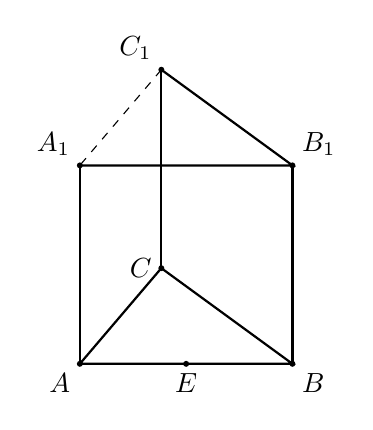
\begin{tikzpicture}[scale=0.9]
  \coordinate (A) at (0,0);
  \coordinate (B) at (3,0);
  \coordinate (C) at (1.15,1.35);
  \coordinate (A1) at (0,2.8);
  \coordinate (B1) at (3,2.8);
  \coordinate (C1) at (1.15,4.15);
  \coordinate (E) at (1.5,0);
  \draw[thick] (A)--(B)--(C)--(A);
  \draw[thick] (A)--(A1) (B)--(B1) (C)--(C1);
  \draw[thick] (A1)--(B1)--(C1);
  \draw[dashed] (C1)--(A1);
  \fill (A) circle (1.2pt) node[below left] {$A$};
  \fill (B) circle (1.2pt) node[below right] {$B$};
  \fill (C) circle (1.2pt) node[left] {$C$};
  \fill (A1) circle (1.2pt) node[above left] {$A_1$};
  \fill (B1) circle (1.2pt) node[above right] {$B_1$};
  \fill (C1) circle (1.2pt) node[above left] {$C_1$};
  \fill (E) circle (1.2pt) node[below] {$E$};
\end{tikzpicture}
\end{center}
\nopagebreak[4]
\Needspace{4\baselineskip}
\textbf{解析}

\gksubpart{(1) 垂直关系}

因 $AC=BC$ 且 $E$ 为 $AB$ 中点，$CE\perp AB$。又 $BB_1\perp$ 底面，故 $CE\perp BB_1$。$AB$、$BB_1$ 是侧面 $ABB_1A_1$ 内相交直线，因此 $CE$ 垂直该侧面，特别有 $CE\perp AB_1$。

\gksubpart{(2) 异面直线距离}

在侧面内从 $E$ 向 $AB_1$ 作垂线 $ED$。由于 $CE$ 垂直侧面，$ED$ 同时垂直 $CE$ 与 $AB_1$，故为公垂线。直角三角形 $ABB_1$ 中 $AE=\sqrt2$、$AB_1=2\sqrt6$，从面积关系得 $ED=AE\cdot BB_1/AB_1=2\sqrt3/3\,\mathrm{cm}$。

\gksubpart{(3) 二面角}

以 $AB_1$ 为交线，$ED$ 在侧面内垂直交线。由 $CE$ 垂直侧面，$CD$ 也垂直 $AB_1$，所以 $\angle CDE$ 是平面角。直角三角形 $CED$ 给出 $\tan\alpha=CE/ED=\sqrt6/2$，进而可得其余弦。

\gkanswer{答案（1）：$CE\perp AB_1$。}

\gkanswer{答案（2）：$\dfrac{2\sqrt3}{3}\,\mathrm{cm}$。}

\gkanswer{答案（3）：$\cos\alpha=\dfrac{\sqrt{10}}5$。}

\end{answer}